
\section{Breadth-first Search and Iterative Deepening}

The execution mechanism of Prolog, resolution with backtracking,
executes one call after another, and backtracks to previous
alternatives upon failure. This causes a depth-first traversal of an
abstract tree of all the possible alternatives of execution. Other
traversals are also possible.

Here we present packages for breadth-first traversal of the
alternatives: executing all possible clauses simultaneously (but
independently of each other). No backtracking is done. Another
possibility is to limit the depth traversal to a certain bound. This
is called iterative deepening.

\subsection{Breadth-first Search}

An alternative to depth-first search is breadth-first search. In
breadth-first search, all the clauses that match a goal are tried at
the same time. The advantages of this form of execution is that
although execution from one clause might loop endlessly, still the
execution of other alternative clauses might keep obtaining solutions.
Consider for example goal \verb+nat(N)+ in:
\begin{quote}
\begin{verbatim}
nat(s(X)):- nat(X).
nat(0).
\end{verbatim}
\end{quote}
%
which has infinitely many solutions: from \verb+N=0+ to
\verb+N=s(...s(0)...)+ (which are intended to represent the natural
numbers). Prolog will loop endlessly, being unable to find any
solution. 

Breadth-first search is enabled with the \verb+bf+ package. Using it,
some predicates can be designated to be executed breadth-first, while
the rest will still be executed depth-first. The predicates to be
executed breadth-first are defined using \verb+<-+ instead of
\verb+:-+ in the neck. Thus:
\begin{quote}
\begin{verbatim}
:- use_package(bf).

nat(s(X))<- nat(X).
nat(0)<- .
\end{verbatim}
\end{quote}
%
will still loop, but will nevertheless keep on returning the
(infinitely many) existing solutions. 

Note the use of \verb+<-+ also in facts (and the space separating it
from the final dot). This is striclty required, since the usual Prolog
facts are considered normal clauses, and therefore will be run
depth-first.

Mixing clauses with \verb+<-+ and with \verb+:-+ in the same predicate
is not advisible. It ends up in having two different predicates: one
which is run breadth-first and another one which is run
depth-first. The results are unpredictable. Thus, be careful with
things like: 
\begin{quote}
\begin{verbatim}
:- use_package(bf).

nat(s(X))<- nat(X).
nat(0).
\end{verbatim}
\end{quote}
%
where the fact is defined for depth-first. The compiler will signal
the problem with a warning message indicating discontiguous clauses for
\verb+nat/1+.

The package \verb+bf+ is implemented as a meta-interpreter of the
program that uses the package. A {\em meta-interpreter} is a program
that executes another program. Because of this, if you debug a program
which uses the package, you will in fact be debugguing the
meta-interpreter, not your program. 

Breadth-first search is a {\em complete} execution procedure: if there
is a solution, breadth-first search will find it. This is because it
tries all possible alternatives simultaneously, and, therefore, it
will reach the solution at some point. The classical depth-first
search of Prolog is not complete. 


\subsection{Breadth-first Search with And-Fairness}

Although being complete, breadth-first search still has a drawback:
execution may loop instead of failing. This is known as an 
{\bf infinite failure}. Endless loops are always a hussle, and it is
better to avoid them. 

The reason for infinite failures in breadth-first search is the lack
of {\em and-fairness}. An execution procedure is and-fair if any goal
that has to be executed is in fact executed at some point in time. For
example, the execution by Prolog of the following code:
\begin{quote}
\begin{verbatim}
p(X):- p(X), q(X).
\end{verbatim}
\end{quote}
%
is not and-fair, since the goal \verb+q(X)+ will never have an
opportunity to execute.

The previous code has no solutions (since there is not a fact for
\verb+p/1+), and this comes up because of the infinite failure
originated, which is independent of and-fairness: whatever the
solution for \verb+q(X)+ was, the endless loop will still be there.

However, in the following code there is no reason for infinite
failure. Execution of \verb+p(f(A))+ can very well terminate with a
finite failure: 
\begin{quote}
\begin{verbatim}
p(f(X)):- p(X), q(X).
p(a).

q(b).
\end{verbatim}
\end{quote}
%
if the execution was and-fair, so that \verb+q(X)+ had an opportunity
to execute. Since the only possible solution for \verb+q(X)+ is
\verb+X=b+, and it is not compatible with the solutions for \verb+p/1+
in the recursive call, there are no solutions in the recursive
clause. The fact does not match, either. Therefore, \verb+p(f(A))+
should (finitely) fail.

However, Prolog will keep on calling the recursive goal and never find
a solution, nor its absence. Exeuction will loop. 

Note that the program also lacks {\em or-fairness}: the fact for
\verb+p/1+ is never given an opportunity to be selected. This is
alleviated with bread-first search:
\begin{quote}
\begin{verbatim}
:- use_package(bf).

p(f(X))<- p(X), q(X).
p(a)<- .

q(b).
\end{verbatim}
\end{quote}
%
but still execution will loop because of the lack of
and-fairness. This is solved by using the and-fair version of the
\verb+bf+ package: 
\begin{quote}
\begin{verbatim}
:- use_package('bf/af').
\end{verbatim}
\end{quote}
%
instead. Execution of \verb+p(f(A))+ will now answer ``no''.

And-fairness is only advisible when the program is pure Prolog. For
example, the execution of:
\begin{quote}
\begin{verbatim}
:- use_package('bf/af').

sumall([],0)<- .
sumall([X|Xs],S)<- sumall(Xs,S0), S is S0+X.
\end{verbatim}
\end{quote}
%
will end up in a run-time error indicating illegal arithmetic
expressions, because the arguments to \verb+is/2+ are not properly
instantiated when it is called. 

The above is due to the way and-fairness is implemented. It ``rotates''
goals so that every one has an opportunity to be executed. Because of
this, the goal \verb-S is S0+X- might be called before the goal
\verb+sumall(Xs,S0)+ produces the required value for \verb+S0+.

\subsection{Depth-first Iterative Deepening}

An alternative computation rule is Depth-first Iterative Deepening.
When this computation rule is used, first goals are expanded only
up to a given depth. I.e., if a goal for predicate \verb+p+ calls a
goal for predicate \verb+q+, and this one a goal for \verb+r+, and so
on, only a certain number of such ``nested'' predicate calls are
executed.  If no solution is found or more solutions are needed by
backtracking, the depth limit is incremented and the goal execution is
continued. 

Although depth-first is not a complete execution procedure, with
regard to space requirements it is much more economical than
breadth-first. This is shown in figure~\ref{fig:spacecom}, where the
abstract trees for a goal for both procedures are shown. The
abstract tree has a branch for every sequence of goal calls that may
arise in a computation, like the chain \verb+p+ calls \verb+q+ calls
\verb+r+ of before. Each node represents the addition of goals to
execute from the clause that has been selected during the
computation.
%% It has two kinds of nodes:
%% and-nodes represent a clause, and its children are the goals of the
%% clause, which are or-nodes, the children of which are, in turn,
%% and-nodes for the applicable clauses.

In breadth-first, all possible clauses (at a certain level of the
tree) are always ``active'', since all are selected. In contrast, for
depth-first only the last clause selected, plus the remaining
alternatives for previously selected clauses are active.
%
From the figure, it can be concluded that depth-first space complexity
is $o(b\cdot d)$ whilst for breadth-first is $o(b^d)$ where $b$ is the
branching factor of the computation tree and $d$ is its depth.

Depth-first iterative deepening with its space economy and overall
breadth-first-like behaviour is therefore a good compromise,
especially since space limitations are, in search problems, usually
most critical. It has been shown by mathematical analysis
\cite{iterative-deepening} that iterative deepening is in a certain
sense in fact optimal with respect to both time and space complexity.
It performs only about b/(b - 1) times as many operations than the
corresponding breadth-first search, whilst the waste of memory is the
same as depth first.

\begin{figure}[htbp]
  \begin{center}
    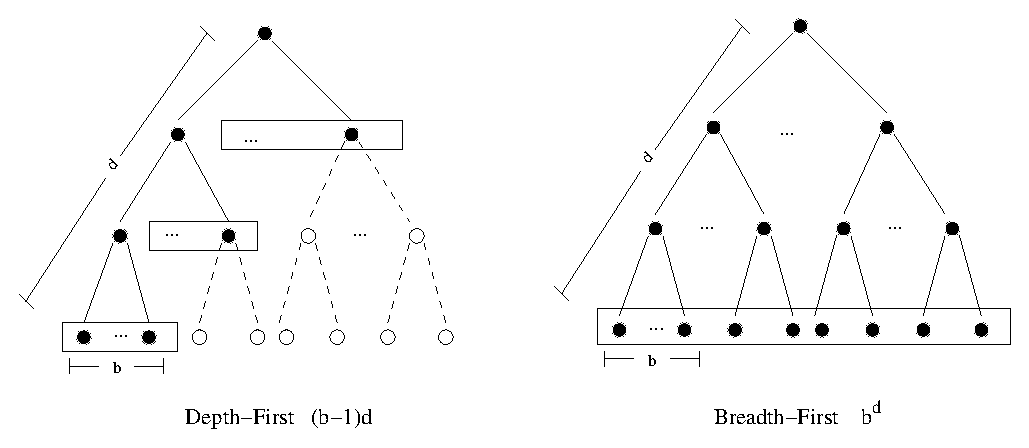
\includegraphics[width=0.8\textwidth]{memusage} 
    \caption{Computation space complexity}
    \label{fig:spacecom}
  \end{center}
\end{figure}

Depth-first iterative deepening search is enabled with the \texttt{id}
package. The predicates to be executed with iterative deepening are
designated using the directive:
\begin{quote}
\texttt{:- iterative(Name, FirstCut, Formula).}
\end{quote}
%
which states than the predicate \texttt{Name}, given as the predicate
spec, will be executed using the iterative deepening rule with an
initial depth limit of \texttt{FirstCut}, depth being incremented by
the predicate \texttt{Formula}. This predicate computes the new depth
using the previous one. It must implement a dilating function, i.e. the
new depth must be greater than the old one. For example, to start with 
depth 5 and increment by 10 you can write:
\begin{quote}
\texttt{:- use\_package(id).}

\texttt{:- iterative(p/1,5,f).}

\texttt{f(X,Y) :- Y is X + 10.}
\end{quote}
%
or if you prefer, using higher order, you can avoid defining a new
predicate as in:
\begin{quote}
\texttt{:- iterative(p/1,5,(\_(X,Y):- Y is X + 10)).}
\end{quote}

Note that the predicate for the formula is assumed to have two
arguments. Only the name, not the arity, is given in the declaration.

You can also use a fourth parameter to set a limiting depth. All goals
below the given depth limit simply fail. Thus, with the following
directive: 
\begin{quote}
\texttt{:- iterative(p/1,5,(\_(X,Y):- Y is X + 10),100).}
\end{quote}
%
all goals deeper than 100 will fail. 

Iterative deepening is enabled for calls that happen within the module
that uses the package. If there is a call to an imported predicate,
this call will reset the depth limit, and therefore, it will be
treated in the usual depth-first fashion. If it was to a predicate
which, in turn, was designated for iterative deepening execution in
its module, then it will be executed in this fashion. But in this case
the depth count will start in 0, so its depth will not be taken into
account for the depth limit of the calling module. Thus, both depth
limits in the two modules will not have any relation at all. This
means that the depth limit set in a module is for chains of goals to
local predicates of the module, only. 

It is possible to preserve the iterative-deepening behavior for calls to
predicates defined in other modules, i.e., to avoid resetting the
depth in calls to imported predicates. These modules should obviously also
use this package. In addition \emph{all} predicates from such modules
should be imported, i.e., the directive \texttt{use\_module/1} should
be used in this case instead of \texttt{use\_module/2}. Otherwise,
calls to predicates outside the module will be treated in the usual
way, as explained above.
